\vspace*{-0.6cm}
\section{Running Example}


\begin{figure}[t]
  \centering
  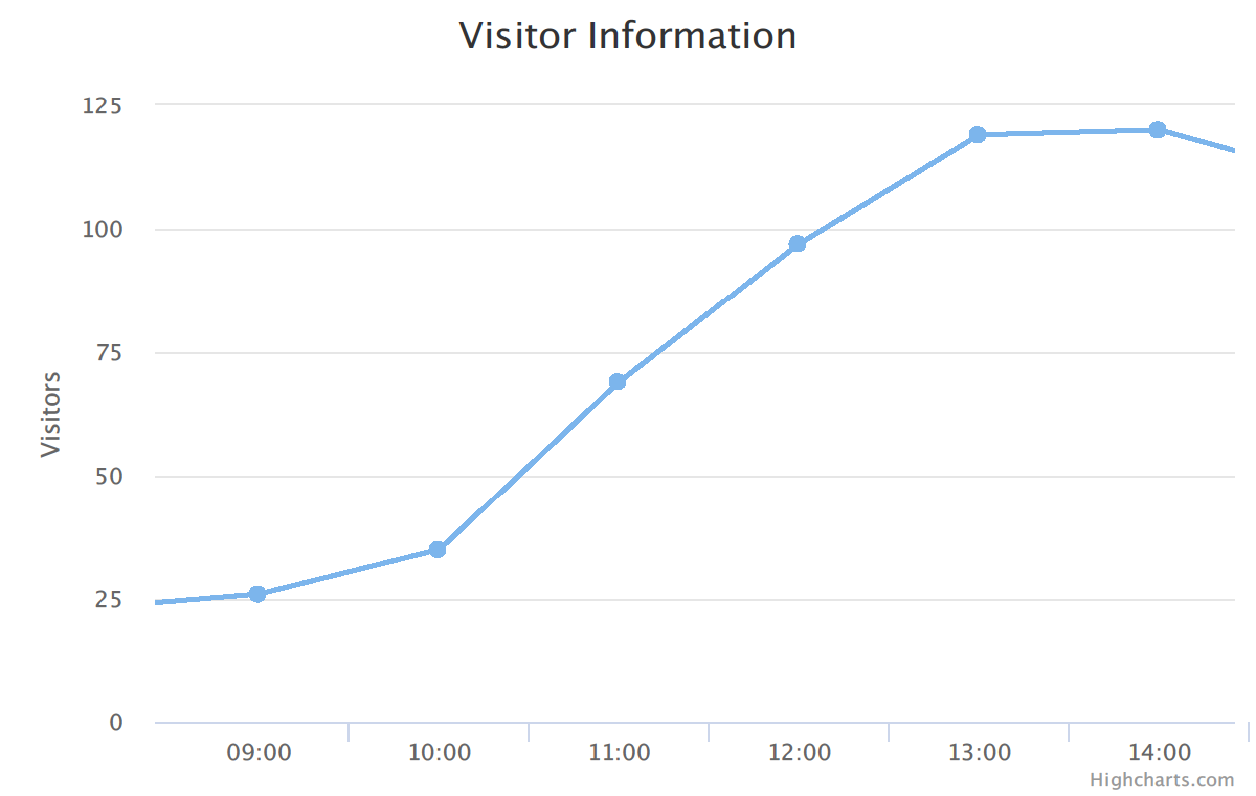
\includegraphics[width=0.8\columnwidth]{figures/first-line.png}
  \caption{Line chart showing visitors per hour}
\label{figure:first-running-example:first-line-chart}
  %\vspace*{\floatsep}% http://tex.stackexchange.com/q/26521/5764
   \vspace*{0.1cm}
  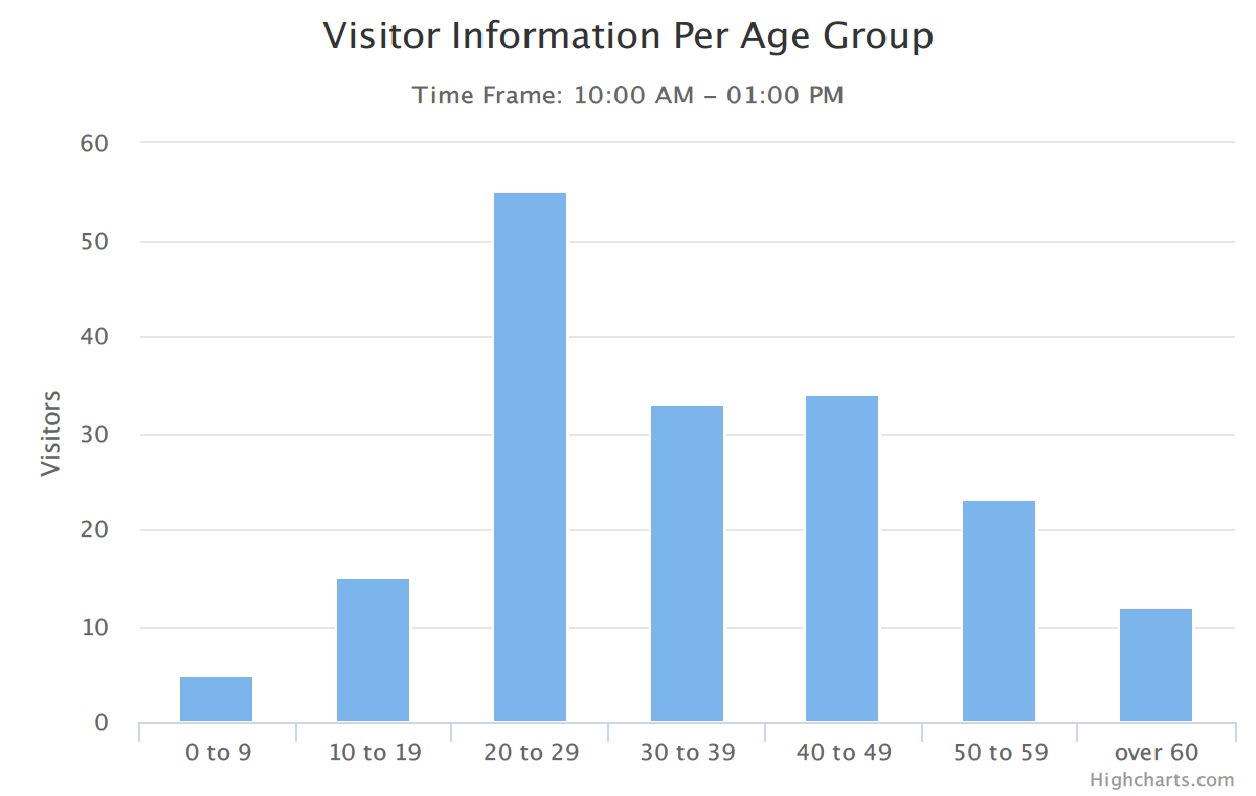
\includegraphics[width=0.8\columnwidth]{figures/first-bar.png}
  \caption{Bar chart showing age groups of visitors}
  \vspace{-10pt}
  \label{figure:first-running-example:first-bar-chart}
  
\end{figure}

\begin{table}
\begin{center}

\begin{tabular}{|c|c|c|c|c|}
\hline 
\multicolumn{5}{|c|}{Page Views} \\ 
\hline 
id & vid & url & time & date \\ 
\hline 
\end{tabular} 

\hfill

\begin{tabular}{|c|c|c|c|c|}
\hline 
\multicolumn{5}{|c|}{Visitors} \\ 
\hline 
vid & name & lastname & username & age \\ 
\hline 
\end{tabular} 

\end{center}
\caption{Schema description of the two tables in our database.}
\label{tab:schema}
\end{table}


In order to illustrate the issues with existing notebooks and describe the extensions in \projname\, we will use the following example of a potential analysis:

\begin{example}
Consider a data analyst, working for a news portal website. The analyst wishes to create a notebook that extracts and presents information about the demographics of the website's reader-base during particular hours. More specifically, the analyst wants to construct a chart showing the number of readers that visit the website during the day; then based on this information, she would like to extract the age groups of the visitors, during various hours of that day and present the results to the portal editor. Figure \ref{figure:first-running-example:first-line-chart} shows the graph that displays the number of visitors per hour in a line chart and Figure \ref{figure:first-running-example:first-bar-chart} displays the age groups of the visitors in a bar chart. By doing this, the analyst can convince the portal editor to publish more articles and advertisements that target particular age groups during hours in which they visit the portal the most, thus maximizing the portal's revenue and reader's satisfaction.
\end{example}

\eat{
\begin{figure}[ht]
  \centering
  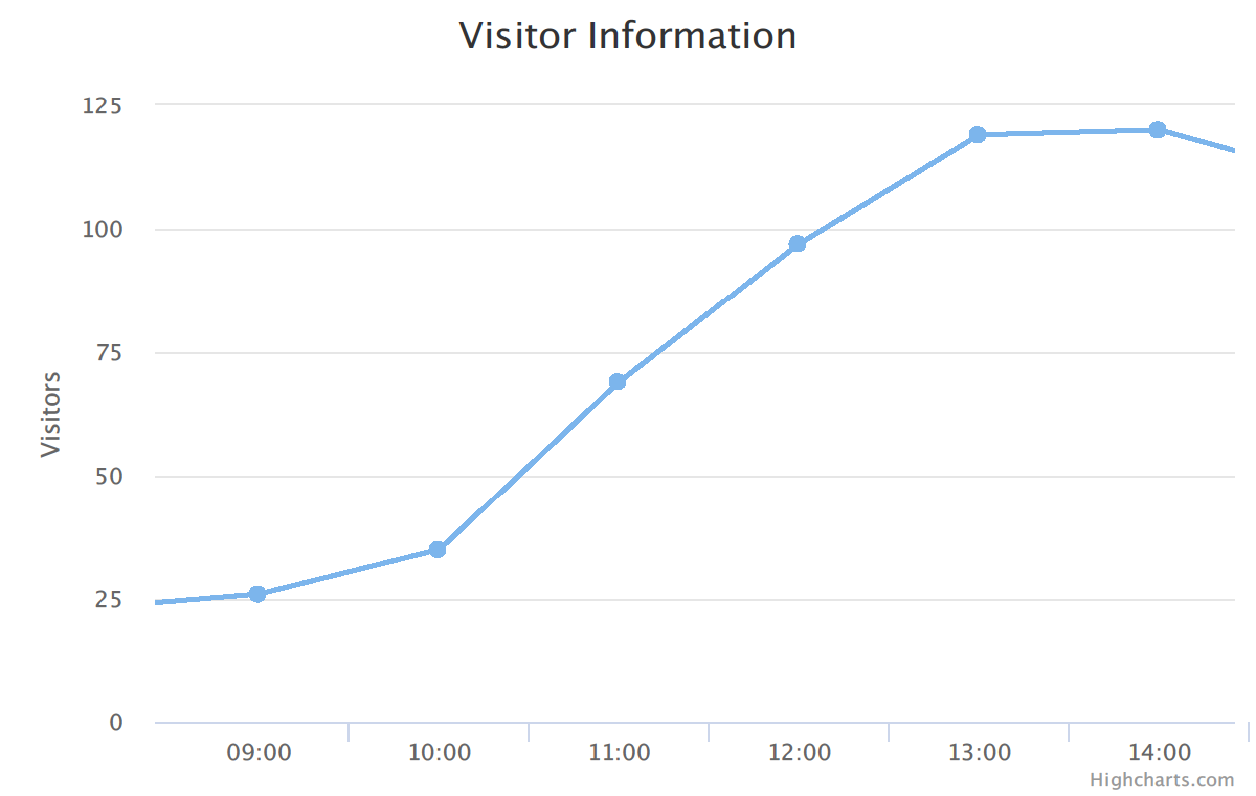
\includegraphics[width=0.8\columnwidth]{figures/first-line.png}
  \caption{Line chart showing visitors per hour}
\label{figure:first-running-example:first-line-chart}
  %\vspace*{\floatsep}% http://tex.stackexchange.com/q/26521/5764
   \vspace*{0.1cm}
  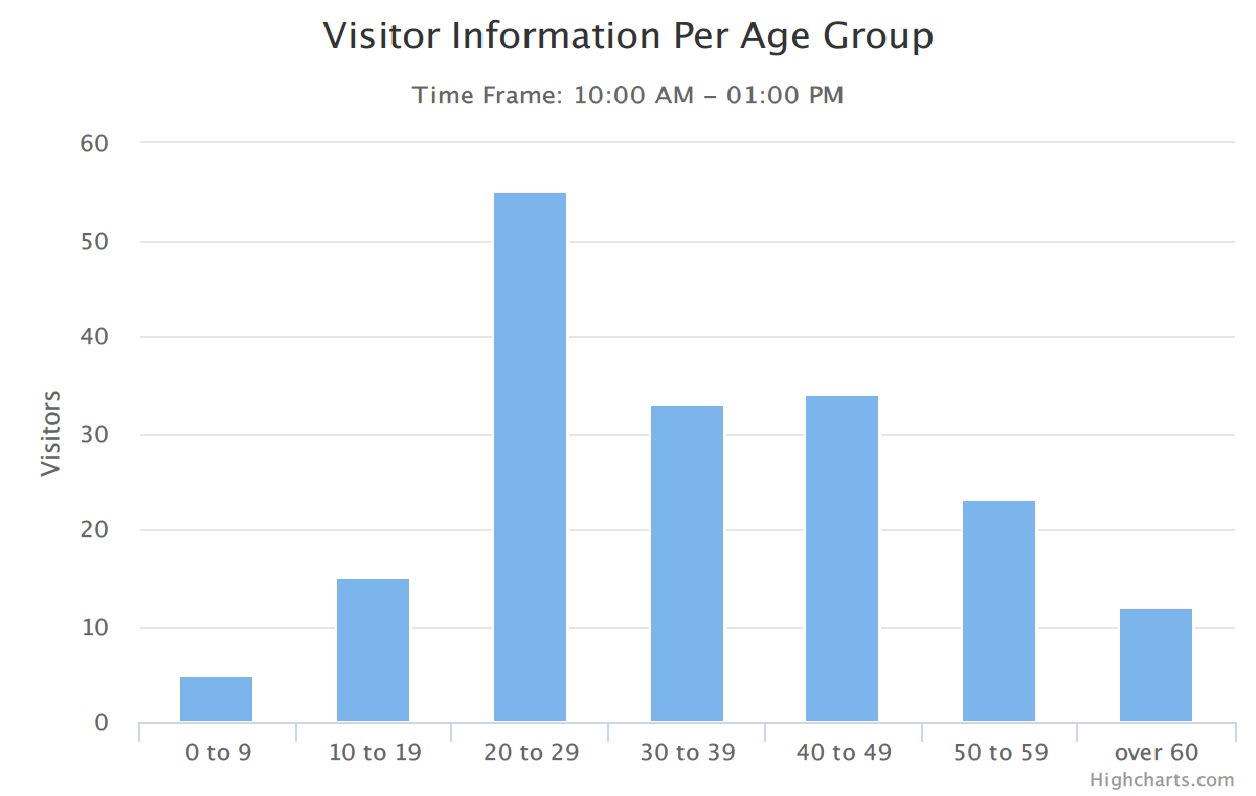
\includegraphics[width=0.8\columnwidth]{figures/first-bar.png}
  \caption{Bar chart showing age groups of visitors}
  \label{figure:first-running-example:first-bar-chart}
\end{figure}
}


For this analysis, we assume that the news portal maintains information about its reader-base in a Postgres database. Table \ref{tab:schema} shows a potential schema, that could be used for storing visitor information. The database contains two tables, namely ``Page Views" and ``Visitors"; table ``Visitors" contains information about each reader, such as the reader id, name, lastname, username and age. The table ``Page Views" maintains a tuple for each visit, and it consists of a visit id, the visitor id (foreign key referencing the visitor), the url of the visited page and the hour and date in which the user visited the website. The reader information could have been retrieved, with their permission, from various social media services (such as Facebook, Google etc). In order to construct this notebook, the data analyst must (a) retrieve  website access information from the database, by joining the two tables on the visitor id (b) generate a plot that shows the number of users that visit the website during the day, (c) issue a query that counts the number of visitors per age group, for each potential set of selected hours, and (d) create a bar chart that shows the number of visitors per age group. 



